\documentclass[11pt, leqno]{article}
\usepackage[margin=0.5in]{geometry}
\usepackage[x11names]{xcolor}
\usepackage{amsfonts,amsmath,amssymb,amsthm}
\usepackage{float}
\usepackage{etoolbox}
\usepackage{ragged2e}
\usepackage{graphicx}
\usepackage{tikz}
\usepackage{pgfplots}
\usepackage{multicol}
\pgfplotsset{compat=1.5}
\author{Nikolai Merritt}
\title{Understanding Calculus for Beginners}
\date{\vspace{-5ex}}
\numberwithin{equation}{section}
\graphicspath{{Images/}}

\begin{document}

\makeatletter
\newif\if@gather@prefix 
\preto\place@tag@gather{% 
	\if@gather@prefix\iftagsleft@ 
	\kern-\gdisplaywidth@ 
	\rlap{\gather@prefix}% 
	\kern\gdisplaywidth@ 
	\fi\fi 
} 
\appto\place@tag@gather{% 
	\if@gather@prefix\iftagsleft@\else 
	\kern-\displaywidth 
	\rlap{\gather@prefix}% 
	\kern\displaywidth 
	\fi\fi 
	\global\@gather@prefixfalse 
} 
\preto\place@tag{% 
	\if@gather@prefix\iftagsleft@ 
	\kern-\gdisplaywidth@ 
	\rlap{\gather@prefix}% 
	\kern\displaywidth@ 
	\fi\fi 
} 
\appto\place@tag{% 
	\if@gather@prefix\iftagsleft@\else 
	\kern-\displaywidth 
	\rlap{\gather@prefix}% 
	\kern\displaywidth 
	\fi\fi 
	\global\@gather@prefixfalse 
} 
\def\math@cr@@@align{%
	\ifst@rred\nonumber\fi
	\if@eqnsw \global\tag@true \fi
	\global\advance\row@\@ne
	\add@amps\maxfields@
	\omit
	\kern-\alignsep@
	\if@gather@prefix\tag@true\fi
	\iftag@
	\setboxz@h{\@lign\strut@{\make@display@tag}}%
	\place@tag
	\fi
	\ifst@rred\else\global\@eqnswtrue\fi
	\global\lineht@\z@
	\cr
}
\newcommand*{\beforetext}[1]{% 
	\ifmeasuring@\else
	\gdef\gather@prefix{#1}% 
	\global\@gather@prefixtrue 
	\fi
} 
\makeatother	
	
\newcommand{\Diff}[1] {\mathop{\text{d}#1}}
\newcommand{\Deriv}[2] {\frac{ \Diff{#1} }{ \Diff{#2} }}
\newcommand{\DelFrac}[2]{\frac{\Delta #1}{\Delta #2}}
\newcommand{\LimDeriv}[2]{ \lim_{\Delta #2 \to 0} \frac{#1(#2 + \Delta #2) - #1(#2)}{\Delta #2} }
\newcommand{\NthDeriv}[3]{\frac{ \text{d}^{#3} #1} {\text{d} #2^{#3}}}
\newcommand{\OutsideDeriv}[2]{\frac{ \text{d} }{ \text{d} #2 } \left( #1 \right)}
\newcommand{\asreq}{\textrm{, as required.} \qed}
\newcommand{\fs}{\, .}
\newcommand{\nn}{\\ \nonumber \\}
\maketitle

\newpage
\tableofcontents

\newpage
\section{Know your Limits}
Imagine that you're watching a live game of basketball, on your TV. Your favourite team's been playing well, but there's only half a minute left, and they're just one point behind. Their lead player gets the ball, spotting a clear path to the opposition's net. He throws the ball towards it as you sit on the edge of your seat, staring intently at the TV screen. Halfway as the ball curves through the air, the connection stutters for a split second, but when it resumes the ball has fallen through the net, and your favourite team's cheering. 
\\ \\
Now, even though you never actually saw what happened in those last few seconds of the game, it doesn't take a genius to figure it out. Just before the connection stuttered, it was looking like the ball was going to fall through the hoop. And, immediately after the connection stuttered, it looked like the ball fell through the hoop too. In fact, if you replayed the last thirty seconds of the match in slow motion, you'd observe that as the time gets closer and closer to the bit where the connection was lost, the ball gets closer and closer to falling into the hoop. And, the closer and closer we get to immediately after the connection was lost, the clearer and clearer it is that the ball fell through the hoop too. So, while you haven't seen for your own eyes what happened at that time, you can still have an incredibly accurate idea of what went on.  
\\ \\
This very intuitive way of thinking can be applied not only to everyday life, but to great effect in mathematics too. Imagine that Jim is in charge of monitoring the daily water level at the river Thames, and it so happens that the rise of millimetres of water height, in terms of times passed in hours, is
\begin{align*}
\text{rise in water level} &= \frac{(t + 5) \ (t - 12)}{t - 12}.
\end{align*}
\\ \\
If Jim called us 8 hours in and asked us how what the rise in water level was, we could simply put 8 into our formula to get:
\begin{align*}
\text{rise in water level} &= \frac{(8 + 5) \ (8 - 12)}{8 - 12} = \frac{13 \times -4}{-4} = 13 \ \text{mm.}
\end{align*}
\\ \\ 
But here's the problem: what if Jim then wanted us to check the rise 12 hours in? Simply putting 12 into our formula would give us:
\begin{align*}
\text{rise in water level} = \frac{(12 + 5) \ (12 - 12)}{12 - 12} = \frac{17 \times 0}{0}.
\end{align*}
And we don't know the answer to this question. No one knows what anything divided by zero is. 
\\ \\
However, we can still offer Jim an incredibly good estimate to how much the Thames' water level has risen. Like in our earlier basketball scenario, we can look at what happens when the time passed gets closer and closer to 12 and make a guess from that. \(t = 11.5\) seems to be as good a start as any:
\begin{align*}
\text{rise in water level} = \frac{(11.5 + 5) \ (11.5 - 12)}{11.5 - 12} = \frac{16.5 \times -0.5}{-0.5} = 16.5 \, \text{mm.}
\end{align*}
\\ Now let's get closer. \(t = 11.9\) will give us a more accurate guess:
\begin{align*}
\text{rise in water level} = \frac{(11.9 + 5) \ (11.9 - 12)}{11.9 - 12} = \frac{16.9 \times -0.1}{-0.1} = 16.9 \, \text{mm.}
\end{align*}
\\ And if we wanted to get even more accurate still, when \(t = 11.999\):
\begin{align*}
\text{rise in water level} = \frac{(11.999 + 5) \ (11.999 - 12)}{11.999 - 12} = \frac{16.999 \times -0.0001}{-0.0001} = 16.999 \ \text{mm.}
\end{align*}
\\ Just to be sure, let's check the water level rise immediately after 12 minutes. If everything goes well, this should give us an answer very close to 17 too:
\begin{align*}
\text{rise in water level} = \frac{(12.0001 + 5) \ (12.0001 - 12)}{12.0001 - 12} = \frac{17.0001 \times 0.0001}{0.0001} = 17.0001 \, \text{mm.}
\end{align*}
\\ So we can safely say that, as the time passed gets closer and closer to 12 minutes, our answer gets closer and closer to 17 mm. In other words, the approaching value of our water level rise is 17, as \(t\) approaches 12.
\\ For whatever reason, mathematicians use the word ``limiting" instead of ``approaching". They'd say that the \textbf{limiting value} -- or ``limit" for short -- of our answer is 17, as \(t\) gets closer to 12.
\\ \\ Because the idea of finding a limit is such a useful tool, mathematicians have also invented their own notation for it. Instead of having to write out the previous sentence, they would write:
\begin{flalign*}
\lim_{t \to 12} \left( \text{rise in water level} \right) = 17 \\
\intertext{or } \lim_{t \to 12} \frac{(t+5) \ (t - 12)}{t-12} = 17.
\end{flalign*}
\\ Now that we've got the jargon out the way, you may be wondering how we can be so sure our limit is 17 \textit{exactly}? What if our rise actually approaches, say, 16.9998, 17.0002, or 17 \( + \frac{2}{8653}\)? While our answer of ``some number pretty damn close to 17" should do just fine for this simple scenario, knowing if some function limits to, say, \(\pi\), with all its uses and shortcuts, instead of 3.1416, can be vital for more important situations. This is why most limits are solved algebraically, instead of plugging in numbers and watching what happens. This allows for far more precision and rigour.  
\\ \\ Thankfully, just like how fundamentally simple the idea of a limit is, so are the ways in which it can be used. Unlike a concrete function like \(\sin(x)\), a limit is more like a concept, and so is a bit more malleable. When we're adding, subtracting, multiplying or dividing different functions, it doesn't matter whether we look at what they approach together, or considered individually; it makes no difference to our answer. Or, in mathematical terms...
\begin{flalign*}
\intertext{For any functions \(f(x)\) and \(g(x)\), and any number \(c\), }
\lim_{x \to c} \left[ f(x) + g(x) \right] &= \lim_{x \to c} f(x) \ + \ \lim_{x \to c} g(x) \\ \\
\lim_{x \to c} \left[ f(x) - g(x) \right] &= \lim_{x \to c} f(x) \ - \ \lim_{x \to c} g(x) \\ \\
\lim_{x \to c} \left[ f(x) \times g(x) \right] &= \lim_{x \to c} f(x) \ \times \ \lim_{x \to c} g(x) \\ \\
\lim_{x \to c} \, \frac{f(x)}{g(x)} &= \frac{\lim\limits_{x \to c} f(x)}{\lim\limits_{x \to c} g(x)}
\end{flalign*}
\\ With these four properties made clear, we can easily start to demonstrate how we could work out the limit for our water level equation algebraically:
\begin{align*}
\lim_{t \to 12} \frac{(t + 5) \ (t - 12)}{t - 12} &= \lim_{t \to 12} \left( \frac{t - 12}{t - 12} \ (t + 5) \right) \\ \\
 &= \lim_{t \to 12} \left(\frac{t - 12}{t - 12}\right) \times \lim_{t \to 12} (t + 5).
\end{align*}
\\ Note that we're taking the limit as \(t\) approaches 12. Similar to our estimation in the mystery connection loss in our basketball scenario, we see what happens as \(t\) \textit{approaches} 12, not when \(t\) \textit{is} 12 So, cancelling both sides of the fraction won't be dividing by zero. This means:
\begin{align*}
\lim_{t \to 12} \frac{(t + 5) \ (t - 12)}{t - 12} &= \lim_{t \to 12} 1 \times \lim_{t \to 12} \left( t + 5 \right). \\
\end{align*}
Great! Now we've reduced it to a simple common-sense question. Our first limit on the right hand side doesn't care what value \(t\) is. Whether \(t = \) 11.9, 15, or a million, it doesn't make a difference; no matter what, \(1 = 1\). And it's equally obvious that, if we make \(t\) get closer and closer to 12, \(t + 5\) will get closer and closer to 17. So we have:
\begin{align*}
\lim_{t \to 12} \frac{(t + 5) \ (t - 12)}{t - 12} &= 1 \times 17 \\
&= 17.
\end{align*}
\\ So, now we can say with almost 100\% certainty that, despite the nasty division by zero, the increase in the water level at 12 minutes in is exactly 17. Of course, this is only a humble little demonstration of the power of limits, but hopefully you can imagine how limits can be used to find incredibly accurate estimates for otherwise unknowable answers. In fact, limits form the bedrock of Calculus, another extremely powerful and versatile tool in mathematics. 
\\ \\ In the next section we will explore the most famous limit ever: the derivative. However, it's vital to be as comfortable with each topic as possible before moving on to the next one. This book goes through topics extremely fast, so it'll be easy to be swept off your feet otherwise. Completing the 8 questions overleaf should be enough. Worked solutions are at the back of the book.
\newpage
Prove the following propositions:
\begin{flalign}
	\lim_{x \to -2} \left(12x^2 + 5 \right) &= 53 \nn
	\lim_{x \to a} \frac{(x + 3) \ (x - a)}{x - a} &= a + 3 \nn
	\lim_{x \to -2} \left( 12 \, \frac{x^2 - 4}{x + 2} \right) &= -48 \nn
	\lim_{h \to 0} \frac{(6 + h)^2 - 36}{h} &= 12 \nn
	\lim_{h \to 0} \ \frac{x}{3-\sqrt{x+9}} &= -6 \nn
	\lim_{U \to 0} \frac{1- \sqrt{1-U^2}}{U} &= 0 \nn
	\lim_{\alpha \to 0} \frac{1- \sqrt{1-\alpha^3}}{\alpha^3} &= \frac{1}{2} \nn
	\lim_{\psi \to 0} \frac{\sqrt{a + \psi} - \sqrt{a}}{\psi} &= \frac{\sqrt{a}}{2a} 
\end{flalign}

\newpage
\section{Deriving the Derivative}
\subsection{Introduction to the concept}
It's often very useful to know the rate of change of something. An obvious example is velocity; without being able to how fast an object is going -- or, in other words, the rate of change of its distance vs time -- we'd all die in car crashes on our first day of driving. And there are many more examples: how fast diseases spread, the ebb and flow of the stock market, and the growth of populations, to name a few. However, the first example is probably the simplest.
\\ \\ Let's picture a scenario to demonstrate this. Imagine the Leibniz family is going to England on holiday. Arriving at Heathrow airport, they take a taxi to their hotel in central London -- a 20 minute journey. Their taxi driver is driving quite erratically to beat the London traffic. So it so happens that their distance in metres from Heathrow, \(s\), in terms of time passed in minutes, \(t\), is
\begin{flalign*}
	s(t) &= t^2 \ \text{ when } 0 \leq t \leq 20.
\end{flalign*}
Given this, it's very easy to find their average velocity across any section of their journey. Say we wanted to find their average velocity for the last 15 minutes. We know that 
\begin{flalign*}
	\text{avg velocity} &= \DelFrac{s}{t} = \frac{\text{new dist} - \text{old dist}}{\text{new time} - \text{old time}} \fs \\ \\
	\intertext{By convention, let's refer to the starting time as \(t\) and our change in time as \(\Delta t\) \newline So, we have:} &
	\begin{array} {l l l}
		\text{old time} = t & \Rightarrow & \text{old dist} = t^2 \\
		\text{new time} = t + \Delta t & \Rightarrow & \text{new dist} = (t + \Delta t)^2
	\end{array}
	\intertext{So, using this,}
	\text{avg velocity} &= \frac{(t + \Delta t)^2 - t^2}{\Delta t} \\
	\intertext{Using \(t = 5\) and \(\Delta t = 15\), we get:}
	\text{avg velocity} &= \frac{(5 + 15)^2 - 5^2}{15} \\ \\
	&= \frac{375}{15} \\ \\
	&= 25 \fs
\end{flalign*}
\\ \\However in reality, we rarely care about someone's average velocity across a time period. It's far more common that we want to find the velocity \textbf{now}, at a single point in time. In other words, when there is no change in time. When \(\Delta t = 0\). 
\\ \\ Unfortunately, we can't just plug in 0 for \(\Delta t\) and read off our answer. That would mean dividing by 0, and no one knows how to work out an answer that way. Instead, as with our previous problem, our only option is to use the method of limits and see what value our velocity approaches as we let \(\Delta t\) approach 0. 
\\ \\ Let's give a name to our velocity at a single point. We'll call this $\Deriv{s}{t} \fs$ Now, using our limit definition, we have:
\begin{flalign*}
	\Deriv{s}{t} &= \lim_{\Delta t \to 0} \DelFrac{s}{t} \\ \\
	&= \lim_{\Delta t \to 0} \frac{(t + \Delta t)^2 - t^2}{\Delta t} \\ \\
	&= \lim_{\Delta t \to 0} \frac{t^2 + 2t \, \Delta t + (\Delta t)^2 - t^2}{\Delta t} \\ \\
	&= \lim_{\Delta t \to 0} \frac{2t \, \Delta t + (\Delta t)^2}{\Delta t} \fs
	\intertext{Again, because \(\Delta t\) \textit{approaches} 0, not \textit{equals} 0, we can divide both sides by \(\Delta t\) just fine. So we have:}
	\Deriv{s}{t} &= \lim_{\Delta t \to 0} \left(2t + \Delta t \right) \\ \\
	&= 2t \, , \text{ by common sense.}
\end{flalign*}
And there we have it. A general-use formula for the family's velocity at any minute \(t\). Of course, \(\Deriv{s}{t} = 2t\) only when \(s(t) = t^2\). But this limit method could be used to find the rate of change of any function. 
\\ \\Now for some jargon. Our instant rate of change in $s$, $\Deriv{s}{t}$ is called the derivative of $s$. And the method we just used to find it, by dealing with tiny differences in $s$ and $t$, is called differentiation. Note that $\Deriv{s}{t}$ is \textbf{not} actually a fraction. It's the \textbf{limit} of a fraction, yes, but $\Diff{s}$ and $\Diff{t}$ don't make any sense by themselves. For reasons we'll see later on, it's useful to write derivatives the same way we write fractions. But that's as far as it goes.
%
\\ \\ Now that we have found out that every \footnotemark function has a derivative, let's investigate this further. Patterns come up in all sorts of surprising places in maths, and fortunately, there's a pattern for the derivative of polynomials. To observe this, let's collect some information -- starting with \(x^3\)...
\begin{flalign*}
	\Deriv{(x^3)}{x} &= \lim_{\Delta x \to 0} \DelFrac{(x^3)}{x} \\ \\
	&= \lim_{\Delta x \to 0} \frac{(x + \Delta x)^3 - x^3}{\Delta x} \\ \\
	&= \lim_{\Delta x \to 0} \frac{x^3 + 3x^2 \, \Delta x + 3x (\Delta x)^2  + (\Delta x)^3 - x^3}{\Delta x} \\ \\
	&= \lim_{\Delta x \to 0} \frac{3x^2 \, \Delta x + 3x (\Delta x)^2 + (\Delta x)^3}{\Delta x} \\ \\
	&= \lim_{\Delta x \to 0} \left[ 3x^2 + 3x \, \Delta x + (\Delta x)^2 \right] \fs
	\intertext{Now we have reduced it to a common sense level. As \(\Delta x\) gets closer and closer to 0, the \(3x \, \Delta x\) and \((\Delta x)^2 \) terms will get closer and closer to 0 too. So, we finally have, }
	\Deriv{(x^3)}{x} &= 3x^2 \fs
	\intertext{Through the same process, which I have hidden for brevity, we can arrive at}
	\Deriv{(x^4)}{x} &= 4x^3
	\intertext{and}
	\Deriv{(x^5)}{x} &= 5x^4 \fs
	%
	\intertext{That should be enough information. Now let's lay present our findings.}
	& \def\arraystretch{1.5}
	\begin{array} {|l | l l|}
		\hline
		f(x) & & \Deriv{f}{x} \\ \hline \hline
		x^2 & & 2x^1 \\ \hline
		x^3 & & 3x^2 \\ \hline
		x^4 & & 4x^3 \\ \hline
		x^5 & & 5x^4 \\ \hline
	\end{array}
	\intertext{As we can see, the derivative of a power function seems to be the function multiplied by its power, then its own power is reduced by 1. Or, in mathematical notation, }
	\Deriv{(x^n)}{x} &\equiv nx^{n-1} \ \ \text{for any } n \fs
	\intertext{Notice how I showed this through a pattern, not by proving it. That's because proving it for any natural \(n\) is easy enough for you to do it! And as for \textbf{any} \(n\), it's definitely possible, but only by techniques in the next section. }
\end{flalign*}
\footnotetext{Strictly speaking, only functions that are continuous -- that is, don't have any sharp bends, vertical tangents, or gaps at any point in their range -- are differentialbe. But pretty much every function you've seen is like that.}
\newpage
\begin{flalign}
	\intertext{Prove the following derivative rules. You may, without proof, quote the Binomial Theorem if required.}
	\Deriv{\left[ f(x) + g(x) \right]}{x} & \equiv \Deriv{f}{x} + \Deriv{g}{x} \nn
	\Deriv{\left[ k \cdot f(x) \right] }{x} & \equiv k \, \Deriv{f}{x}  \ \text{ for any constant } k \\\nonumber \\
	\Deriv{k}{x} &\equiv 0 \ \text{ for any constant } k \nn
	\Deriv{(kx^n)}{x} & \equiv nkx^{n-1} \ \text{for any constant } k \text{ and any natural number } n \\ \nonumber
	%
	\intertext{Hence find the following derivatives.}
	\Deriv{\left(12x^3 + 3x^2\right)}{x} \nn
	\Deriv{\left(9y^2 - 2y^5 + 3y\right)}{y} \nn
	\Deriv{ \left(7u^3 + 3u^2 - 2u + 12\right)}{u} \nn
	\Deriv{\left( 8\phi^{12} + 3\phi^{10} + 9\phi^2 - 17 \right)}{\phi} \nn
	%
	\intertext{Let} \nonumber \nolinebreak
	\frac{\textrm{d}}{\textrm{d}x} \left( f \right) &\equiv \Deriv{f}{x}
	\intertext{And let} \nonumber \nolinebreak
	\NthDeriv{f}{x}{2} &\equiv \frac{\text{d}}{\text{d}x} \left( \Deriv{f}{x} \right) \ \equiv \ \Deriv{\left( \Deriv{f}{x} \right)}{x} \\ \nonumber
	\intertext{Hence find} 
	\NthDeriv{(x^3 + 2x^2 + 3x + 1)}{x}{2} \nn
	\NthDeriv{(3z^4 + 2z^3 + 3z)}{z}{2}
\end{flalign}
\newpage
\subsection{The chain rule: the mother of all rules}
Before we can proceed any further with derivatives, we must first understand the chain rule. It forms the foundation of so many things: finding derivatives of nested functions, integration by u-substitution, implicit differentiation, solving differential equations, parametric differentiation, and the list goes on... With something so useful, you'd think it's incredibly complicated, but that couldn't be further than the truth. \nn
First off, let's look at a slightly different way to define a derivative. As with our last way, we start by considering two points along the x-axis, which we shall call $x$ and $p$. Visually, we have: \nn 

\begin{tikzpicture}
	\begin{axis} [
		axis lines = left,
		xlabel = $x$,
		ylabel = $y$,				
	]
	\addplot [color = cyan, domain = 0: 20, very thick] {x^2};	
	\pgfplotsset{ticks = none};
	\draw [red] (axis cs: 10, 0) -- (axis cs: 10, 10^2);
	\node [
		label = {
			[left, red, yshift = 2.1ex, xshift = 0.3em] 180: {$x$}
		},
		circle,
		fill,
		inner sep = 0.2pt,
	]
	at (axis cs: 10, 3) {};
	\draw [red](axis cs: 15, 0) -- (axis cs: 15, 15^2);
	\node [
		label = {
			[left, red, yshift = 2.1ex, xshift = 0.3em] 180: {$p$}
		},
		circle,
		fill,
		inner sep = 0.2pt,
	]
	at (axis cs: 15, 3) {};
	\draw [<->, color = magenta](axis cs: 10.5, 90) -- node[above] {$\Delta x$} (axis cs: 14.5, 90);
	\end{axis}
\end{tikzpicture} \nn
Traditionally, we'd let their distance, $\Delta x$, go to 0. But clearly, saying ``let's the distance between $x$ and $p$ go to 0" is the same thing as saying ``let $x$ get closer and closer to $p$". So we have two identical ways of writing a derivative: 
\begin{flalign}
	 \Deriv{y}{x} &\equiv \LimDeriv{y}{x}  \nn
	\intertext{and }   
	\Deriv{y}{x} &\equiv \lim_{x \to p} \frac{y(x) - y(p)}{x - p} \fs  
	\intertext{More offen than not, it's easiest to use the `` $\Delta x$ to 0 " definition. But sometimes, it's easier to use the ``$x$ to $p$" one. For instance, using that method:}
	 \Deriv{(x^2)}{x} &= \lim_{x \to p} \frac{x^2 - p^2}{x - p}  \nn	
	  &= \lim_{x \to p} \frac{(x - p) \, (x + p)}{x - p}  \nn
	  &= \lim_{x \to p} \left( x + p \right)  \nn
	  	&= 2p 
	\intertext{Or, because $p$ can be anywhere along the x-axis, we can just replace it with $x$ for convenience, like this:}
	  	\Deriv{(x^2)}{x} &= 2x  
	\intertext{Which is a bit nicer than having to deal with $(\Delta x)^2$, dividing by $\Delta x$, etc.}
	\intertext{Now, an example where this definition is a lot nicer is in deriving the chain rule. \newline Consider the chain function}
	  & z(y(x))   \nn
	\text{For example }   z(y) &= y^3 \ \text{ and } \ y(x) + x^2 + 3   \nn
	\text{Would give us }   z &= (x^2 + 3)^3  \nn
	\intertext{Now, how would we find $\Deriv{z}{x}$? \newline Starting with our new definition of a derivative, we have:}
	\Deriv{z}{x} &= \lim_{x \to p} \frac{ z(y(x)) - z(y(p)) }{x - p} \nn
	\intertext{Now, we can split this fraction to make it nicer:}	 
	\Deriv{z}{x} &= \lim_{x \to p} \left[ \frac{z(y(x)) - z(y(p))}{y(x) - y(p)} \cdot \frac{y(x) - y(p)}{x - p} \right] \nn
	&= \lim_{x \to p} \frac{z(y(x)) - z(y(p))}{y(x) - y(p)} \cdot \lim_{x \to p} \frac{y(x) - y(p)}{x - p} \nn
	\intertext{Aha! Our second limit is the derivative of $y$ with respect to $x$. And our first limit is in a similar form too; it's the tiny change in $z$ divided by the tiny change in $y$. In other words, the derivative of $z$ with respect to $y$. So,}
	\Deriv{z}{x} &= \Deriv{z}{y} \, \Deriv{y}{x} \fs
	\intertext{What a lovely result. }
\end{flalign}
\nn

\newpage
\section{The Integral: an integral part of Calculus}
\subsection{Going backwards: the antiderivative}
Previously, we established how to find the rate of change of any polynomial equation. But what if we were given the rate of change, and wanted to get back to the original? For instance, imagine that the police caught someone speeding, and from their analysis, they worked out their velocity, \(v\) at any point in time along their journey as
\begin{align*}
	v(t) &= 12 \, t.
\end{align*} 
Could they then work backwards to find an equation for the criminal's distance? 
\\ \\ To do this, let's start by giving a name to the criminal's displacement. Since referring to it as \(d(t)\) could lead to confusion with \(\text{d}(t)\) -- a completely different concept -- we'll resort to the formal physics notation: \(s(t)\). So, we have
\begin{align*}
v(t) &= \Deriv{s}{t} \fs
\end{align*}
How do we then get to our \(s(t)\)? 
\\ \\ Well, we know that, if \(v(t)\) is a polynomial, then so must \(s(t)\). If we let 
\begin{flalign*}
	s(t) &= kt^n \\
	\intertext{then } \ v(t) &= \Deriv{(kt^n)}{t} = nkt^{n-1}. \\ \\
	\intertext{Putting our power of \(v(t)\) into this, we have} 
	n - 1 &= 1 \\ 
	\Rightarrow n &= 2 \fs \\
	\intertext{And, putting our coefficient of \(v(t)\) in, we get} 
	nk &= 12 \\ 
	\Rightarrow k &= 6 \fs
	\intertext{So we have that \(s\), our ``antiderivative" of \(v\), is \(6t^2 \, \).} \\
	\intertext{Well... almost. It is true that } \Deriv{(6t^2)}{t} &= 12 \, t 
	\intertext{as required. But, consider also} \Deriv{(6t^2 + 1)}{t}, \ \ \Deriv{(6t^2 + 15)}{t} \, , & \text{ and } \ \Deriv{(6t^2 - 50)}{t} \fs
	\intertext{Since the derivative of any constant is 0, surely these also equal \(12 \, t\) ? So our antiderivative doesn't have to \textit{just} be \(6t^2\) . In fact, \(6t^2 + c\) , for any constant \(c\) , would still be correct. To allow for this, we simply add \( + c\) to the end of our antiderivatives. So, we finally have}
	s(t) &= 6t^2 + c
	\intertext{If the police then told us that he was 12 metres into the road when they started recording his distance, we could then use this to solve for \(c\)...}
	\text{When } t &= 0 \, , \ s(t) = 12 \\
	\Rightarrow 6(0)^2 + c &= 12 \\
	\Rightarrow c &= 12
	\intertext{So in this particular example, \(s(t) = 6t^2 + 12\) . It's clear that, in theory \(c\) could have any value, however.}
\end{flalign*}
Now that we've got that example sorted, it's trivial to realise a general method for finding the antiderivative of a polynomial. 
\begin{flalign*}
	\intertext{In general, for any function}
	f(x) &= kx^n
	\intertext{its antiderivative, which we will call \(F(x)\), will be }
	F(x) &= \frac{k}{n+1} \ x^{n + 1} + c \fs
	\intertext{This can be verified easily; }
	\Deriv{F}{x} &= \frac{k}{n+1} \ (n+1) \ x^{(n+1) \, -1} \\ \\
	&= kx^{(n+1) \, -1} \\ \\
	&= kx^n \\ \\
	&= f(x) \ \text{ as required.} \\
\end{flalign*}
This brings us to a close with the antiderivative. As with the other sections, taking a pause and solving polynomial antiderivative questions is highly reccomended before going further. Ideally you should only move on when you're at the stage where you can look at a polynomial expression and instantly say its derivative and antiderivative.
\newpage
\subsection{Finding areas: the Riemann sum}
In mathematics, it's often useful to find the area of a given shape. Whether two- or three-dimensional, this can be done by drawing a diagram, splitting the shape up into a group of manageable sub-shapes, and sum the areas of those. But what if we weren't given any standard shape to work with? What if we we had to find the area under a function curve?\\ \\
Let's say we had the following curve, \(y = f(x)\): \\
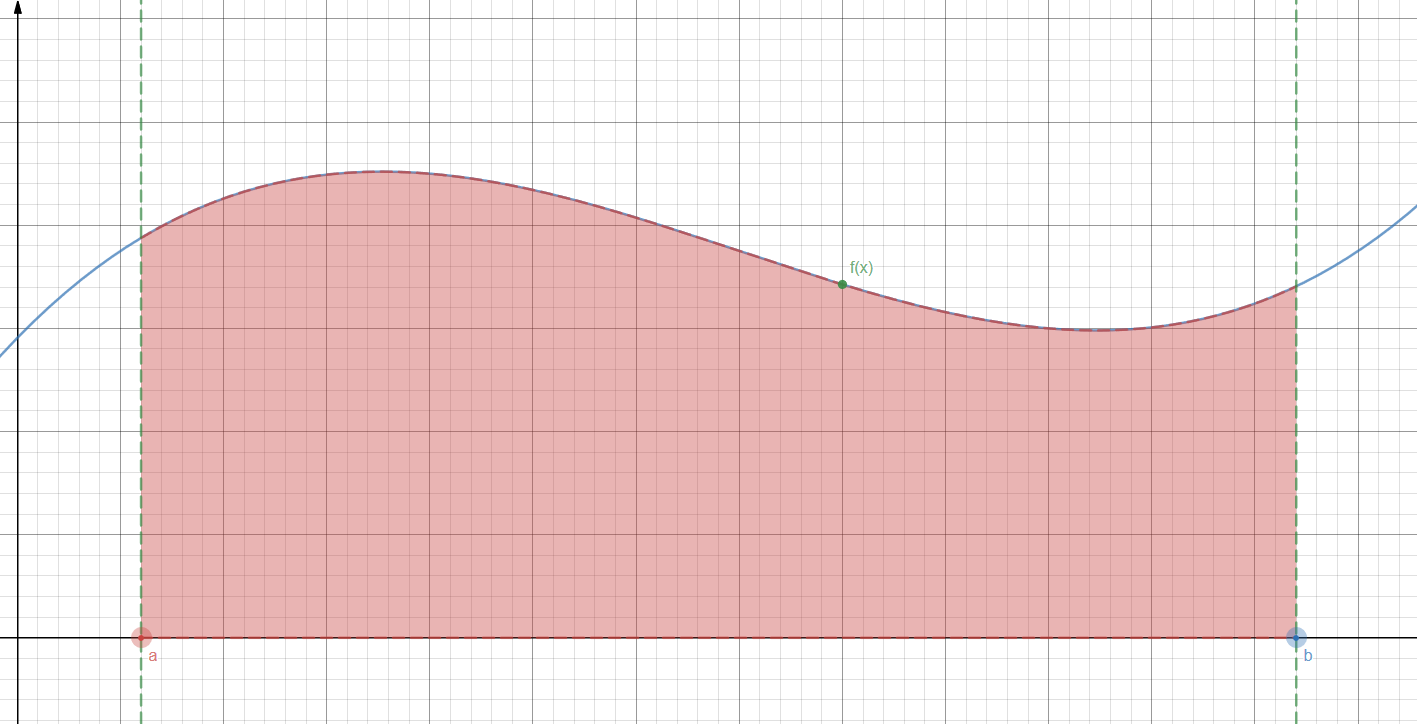
\includegraphics[width=\textwidth]{AreaUnderCurve} \\
How could we go about finding the red area, between the points \(a\) and \(b\)?

\newpage
\section{Solutions}
\begin{flalign*}
	\intertext{1.1}
	\intertext{As \(x\) limits to \(-2\), \ \(12x^2 + 5\) \ limits to \ \(12 \, (-2)^2 + 5\). So we have}
	 \lim_{x \to -2} (12x^2 + 5) &= 12 \, (-2)^2 + 5 \\
	&= 53 \asreq	
	%
	\intertext{1.2}
	\lim_{x \to a} \frac{(x + 3) \ (x - a)}{x - a} &= \lim_{x \to a} \frac{x-a}{x-a} \times \lim_{x \to a} (x + 3) \\ \\
	&= \lim_{x \to a} (1) \times \lim_{x \to a} (x + 3) \\ \\
	&= a + 3 \asreq
	%
	\intertext{1.3}
	\lim_{x \to -2} \left(12 \, \frac{x^2 - 4}{x + 2} \right) &= 12 \lim_{x \to -2} \frac{(x+2) \, (x-2)}{x+2} \\ \\
	&= 12 \lim_{x \to -2} (x-2) \\ \\
	&= 12 \times -4 \ = \ -48 \asreq
	%
	\intertext{1.4}
	\lim_{h \to 0} \frac{(6+h)^2-36}{h} &= \lim_{h \to 0} \frac{36 + 12h + h^2 - 36}{h} \\ \\
	&= \lim_{h \to 0} (12 + h) \\ \\
	&= 12 \asreq
	%
	\intertext{1.5}
	\lim_{h \to 0} \ \frac{x}{3-\sqrt{x+9}} &= \lim_{h \to 0} \frac{x \ (3 + \sqrt{x+9})}{ (3- \sqrt{x+9}) \ (3 + \sqrt{x+9})} \\ \\
	&= \lim_{h \to 0} \frac{x \ (3 + \sqrt{x + 9})}{9 - (x + 9)} \\ \\
	&= \lim_{h \to 0} - \frac{x \ (3 + \sqrt{x + 9})}{x} \\ \\
	&= \lim_{h \to 0} - (3 + \sqrt{x + 9}) \\ \\
	&= -6 \asreq
	%
	\intertext{1.6}		
	\lim_{U \to 0} \frac{1- \sqrt{1-U^2}}{U} &= \lim_{U \to 0} \frac{(1 - \sqrt{1-U^2}) \ (1 + \sqrt{1-U^2}}{U \ (1+\sqrt{1-U^2})} \\ \\
	&= \lim_{U \to 0} \ \frac{1 - 1 + U^2)}{U \ (1 + \sqrt{1-U^2})} \\ \\
	&= \lim_{U \to 0} \ \frac{U}{1+\sqrt{1-U^2}} \\ \\	
	&= \frac{0}{2} = 0 \asreq
	%
	\intertext{1.7}
	\intertext{Similarly to 1.6, }
	\lim_{\alpha \to 0} \frac{1- \sqrt{1-\alpha^3}}{\alpha^3} &= \lim_{\alpha \to 0} \ \frac{1 - (1-\alpha^3)}{a^3 \ (1 + \sqrt{1 + \alpha^3})} \\ \\
	&= \lim_{\alpha \to 0} \ \frac{1}{1 + \sqrt{1 + \alpha^3}} \\ \\
	&= \frac{1}{2} \asreq
	%
	\intertext{1.8}
	\lim_{\psi \to 0} \frac{\sqrt{a + \psi} - \sqrt{a}}{\psi} &= \lim_{\psi \to 0} \frac{(\sqrt{a + \psi} - \sqrt{a}) \ (\sqrt{a + \psi} + \sqrt{a})}{\psi \ (\sqrt{a + \psi} + \sqrt{a})} \\ \\
	&= \lim_{\psi \to 0} \ \frac{a + \psi - a}{\psi \ (\sqrt{a + \psi} + \sqrt{a})} \\ \\
	&= \lim_{\psi \to 0} \frac{1}{\sqrt{a + \psi} + \sqrt{a}} \\ \\
	&= \frac{1}{2\sqrt{a}} \\ \\
	&= \frac{\sqrt{a}}{2a} \asreq
	%
	\intertext{2.1}
	\Deriv{\left[ f(x) + g(x) \right]}{x} & \equiv \lim_{\Delta x \to 0} \frac{f(x + \Delta x) + g(x + \Delta x) - \left[ f(x) + g(x) \right] }\Delta{x} \\ \\
	&\equiv \lim_{\Delta x \to 0} \frac{f(x + \Delta x) - f(x) + g(x + \Delta x) - g(x)}{\Delta x} \\ \\
	&\equiv \lim_{\Delta x \to 0} \frac{f(x + \Delta x) - f(x)}{\Delta x} \ + \ \lim_{\Delta x \to 0} \frac{g(x + \Delta x) - g(x)}{\Delta x} \\ \\
	&\equiv \Deriv{f}{x} + \Deriv{g}{x} \asreq
	%
	\intertext{2.2}
	\Deriv{\left[ k \cdot f(x) \right]}{x} &\equiv \LimDeriv{k \cdot f}{x} \\ \\
	&\equiv \lim_{\Delta x \to 0} k \cdot \LimDeriv{f}{x} \\ \\
	&\equiv k \cdot \LimDeriv{f}{x} \\ \\
	&\equiv k \cdot \Deriv{f}{x} \asreq
	%
	\intertext{2.3}
	\intertext{Consider the function \(f(x) = k\), where \(k\) is any constant. Now, }
	\Deriv{f}{x} &= \LimDeriv{f}{x} \\ \\
	&= \lim_{\Delta x \to 0} \frac{k - k}{\Delta x} \\ \\
	\intertext{Observe that the numerator is 0. Thus, our limit is already 0 before we even evaluate the limit.}
	\therefore{} \Deriv{k}{x} &\equiv 0 \ \text{ for any constant } k \asreq
	%
	\intertext{2.4}
	\intertext{Consider the derivative}
	\Deriv{(x^n)}{x} &\ \text{for any natural number } n
	\intertext{Now, }
	\Deriv{(x^n)}{x} &\equiv \lim_{h \to 0} \frac{(x + h)^n - x^n}{h} \\ \\
	\intertext{Note that \(h\) is being used instead of \(\Delta x\) purely to make the next line tidier. \newline By the Binomial Theorem, we can expand the brackets to get}
	\Deriv{(x^n)}{x} &\equiv \lim_{h \to 0} \frac{ x^n + n \, h \, x^{n-1} + \binom{n}{2} \, x^{n-2} \, h^2 + \binom{n}{3} \, x^{n-3} \, h^3 + \binom{n}{4} \, x^{n-4} \, h^4 + \dotsc +  n \, x \, h^{n-1} + \, h^n - x^n}{h} \\ \\
	&\equiv \lim_{h \to 0} \left[ n \, x^{x-1} + \binom{n}{2} \, x^{n-2} \, h + \binom{n}{3} \, x^{n-3} \, h^2 + \dotsc + h^{n-1} \right] \\ \\
	&\equiv n \, x^{n-1}
	\intertext{Therefore, by 2.2, }
	\Deriv{(kx^n)}{x} &\equiv k \, n \, x^{n-1} \asreq
	%
	\intertext{2.5}
	\intertext{By 2.1,}
	\Deriv{\left(12x^3 + 3x^2\right)}{x} &= \Deriv{(12x^3)}{x} + \Deriv{(3x^2)}{x} \\ \\
	\intertext{And by 2.2,}
	\Deriv{\left(12x^3 + 3x^2\right)}{x} &= 12 \, \Deriv{(x^3)}{x} + 3 \, \Deriv{(x^2)}{x} \\ \\
	&= 12 \cdot 3x^2 + 3 \cdot 2x \\ \\
	&= 36x^2 + 6x
	%
	\intertext{2.6}
	\intertext{Similarly, }
	\Deriv{\left(9y^2 - 2y^5 + 3y\right)}{y} &= 18y - 10y^4 + 3y^0 \\ \\
	&= 18y - 10y^4 + 3
	%
	\intertext{2.7}
	\Deriv{ \left(7u^3 + 3u^2 - 2u + 12\right)}{u} &= 21u^2 + 3u - 2 \\ \\
	%
	\intertext{2.8}
	\Deriv{\left( 8\phi^{12} + 3\phi^{10} + 9\phi^2 - 17 \right)}{\phi} &= 96\phi^{11} + 30\phi^9 + 18\phi
	%
	\intertext{2.9}
	\NthDeriv{(x^3 + 2x^2 + 3x + 1)}{x}{2} &= \Deriv{(3x^2 + 4x + 3)}{x} \\ \\
	&= 6x + 4
	%
	\intertext{2.10}
	\NthDeriv{(3z^4 + 2z^3 + 3z)}{z}{2} &= \Deriv{(12z^3 + 6z^2 + 3)}{z} \\ \\
	&= 36z^2 + 12z 
\end{flalign*}
\end{document}

